\documentclass{assignmeownt}
\usepackage{listings}
\usepackage{amsmath}
\usepackage{nccmath}
\usepackage{pdfpages}

\DeclareMathOperator*{\argmax}{arg\,max}
\DeclareMathOperator*{\argmin}{arg\,min}


\coursenumber{05124265}
\coursetitle{Reinforcement Learning}
\title{Exercise 3}
\author{Tal Grossman, 201512282 , Moshe Yelisevitch, 207423104}
\date{10/07/2024}


\begin{document}
\maketitle
\thispagestyle{firststyle}
\section{Theory}
for theroy sections please see hand written solution.

% TODO MOSHE - incldue pdf for question 1

% hand written solution for question 2 
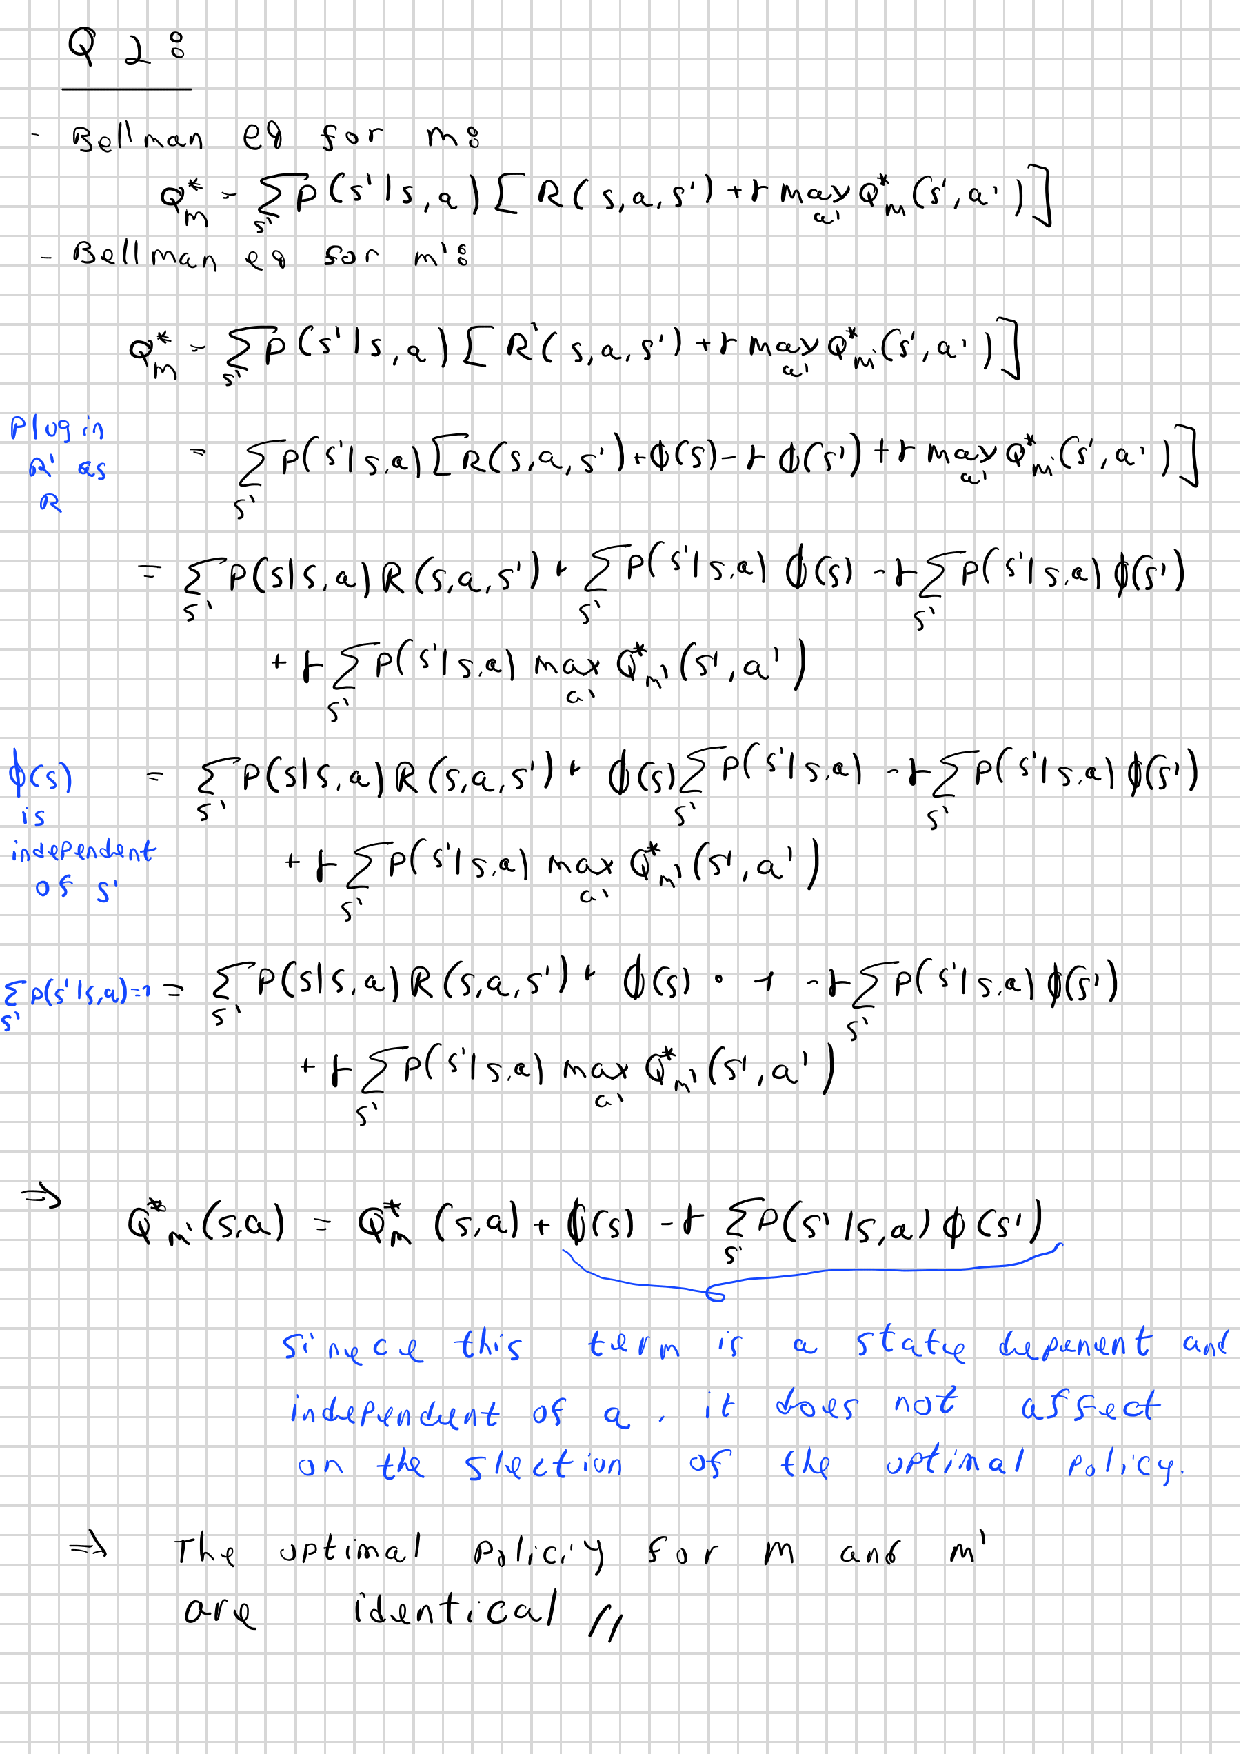
\includepdf[pages=1]{HW3 solution _sol2_4.pdf}

% TODO MOSHE - incldue pdf for question 3

% hand written solution for question 4
\includepdf[pages=2-]{HW3 solution _sol2_4.pdf}

\newpage
\section{Programming}

\subsection{Question 1: Off-Policy Model-Based}
completed in python in the attached file \textbf{control.py}
\newline
In that specific run, it took 263 iterations to converge. The plot of the failure rate is as follows:
\begin{figure}[H]
    \centering
    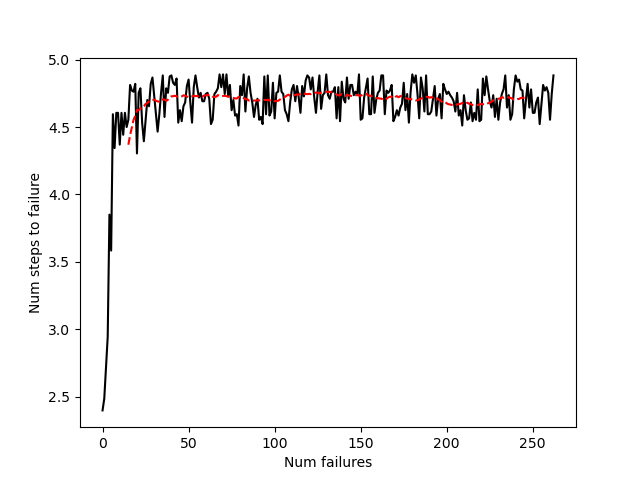
\includegraphics[width=0.3\textwidth]{ex1_263_failure_plot.png}
\end{figure}

\end{document}
